% Chapter Template

\chapter{Related Work} % Main chapter title

\label{Chapter2} % Change X to a consecutive number; for referencing this chapter elsewhere, use \ref{ChapterX}

\lhead{Chapter 2. \emph{Related Work}} % Change X to a consecutive number; this is for the header on each page - perhaps a shortened title

In this chapter, we will discuss the various \textit{deep learning} approaches that have been applied to information retrieval. We initially review the literature that covers the use of pre-trained word embeddings in traditional IR approaches in section~\ref{sec:word_embeddings_ir}. We then discuss  neural network architectures designed specifically for relevance ranking in IR in section~\ref{sec:nn_for_ir}. These models have included insights from traditional retrieval models as neural building blocks. The neural ranking approaches are broadly categorized into two groups: \textit{representation-based} models (section~\ref{sec:representation_based}) and \textit{interaction-based} models (section~\ref{sec:interaction_based})~\citep{Guo2016}. A comparison of the neural ranking model architectures can be observed in Table~\ref{tab:neuir_comparison} and the datasets used in the experimental setups can be seen in Table~\ref{tab:related_work_datasets}.

Finally, in section~\ref{sec:interpretability_ml} we discuss the various \textit{interpretability} approaches that have been used to provide explanations to understand the predictions of machine learning models. We also focus on works that have been proposed recently which apply \textit{interpretability} approaches to understand ranking models in section~\ref{sec:interpretability_in_ir}.

%-----------------------------------------------------
%	SECTION 1
%-----------------------------------------------------
\section{Word Embeddings in IR}
\label{sec:word_embeddings_ir}

In this section, we cover earlier work that incorporated pre-trained word embeddings into traditional ad-hoc retrieval approaches. The papers are categorized into \textit{Implicit}--using vector similarity in the embedding space that is then used in language modelling frameworks and \textit{Explicit}--using word embeddings aggregated for distributed representation of large units of text and then ranking, as discussed in~\citep{Onal_NIR2018}.

\textit{Implicit} In the \textsf{Generalized Language Model} (GLM)~\citep{Ganguly_GLM15} approach they incorporated the semantic similarity between query and document or collection terms measured through the cosine similarity between word embeddings (\texttt{word2vec} CBOW) into the query-likelihood language modelling retrieval approach. They build on the ``noisy channel'' translation model~\citep{Berger99}, where they no longer assume that the query term is generated by sampling independently from either the document or collection but through a generative process that may transform a different term $t'$ from either the document or collection into the observed query term $t$. In the experiments conducted on TREC 6-8 and Robust using Lucene show improvements over both unigram query-likelihood (LM with Jelinek Mercer smoothing) and LDA smoothed LM. 

Similarly, \textsf{Neural Translation Language Model} (NTLM)~\citep{Zuccon15} also integrates word embeddings into the~\cite{Berger99} translation model approach to query-likelihood IR. They estimate the translation probability between terms as the cosine similarity between the terms divided by the sum of the cosine similarities between the translating term and all terms in the vocabulary. Previous state-of-the-art translation models used mutual information (MI) to calculate the translation probabilities. They conduct experiments on TREC datasets AP87-88, WSJ87-92, DOTGOV, and MedTrack and show that NTLM moderately improves over the state-of-the-art (SOTA) MI approaches. The results show that NTLM gets moderate improvements over SOTA based on small improvements over a large number of queries instead of large differences over few queries. Analyzing the various hyper-parameters of the word embeddings shows that NTLM is robust to the choices of embedding dimensionality, context window size, model objective (CBOW vs Skip-gram). Regarding the choice of training corpus for the trained embeddings and its effects on retrieval performance, they show that effectively the best performance is obtained from the same collection on which the retrieval is evaluated but using a different corpus doesn't statistically degrade the retrieval effectiveness.

\textit{Explicit} In the \textsf{Dual Embedding Space Model} (DESM)~\citep{Mitra2016a, Nalisnick:2016}, the authors highlight the importance of retaining both the input and output embeddings from the \texttt{word2vec} model after training. They observed that within the same embedding space (IN or OUT), neighbors are functionally similar words. However, the neighbors of the word using the IN-OUT vector cosine similarity are topically similar words. %\textsf{Topically} similar words are likely to co-occur in a local context, whereas \textsf{functionally} similar words are likely to occur in similar contexts. 
For example, for the term \textit{harvard}, the topically similar terms are the ones that likely co-occur with \textit{harvard} (e.g. \textit{faculty}, \textit{alumini}) and the functionally similar ones are likely to occur in similar contexts (e.g. \textit{yale}, \textit{nyu}). In DESM, query words are represented using the IN vectors and document words with the OUT vectors. A document embedding representation is created by taking an average of the normalized document word vectors. Then, the query-document relevance is computed by taking the average cosine similarity between each query term and document embedding. The word embeddings are generated using \texttt{word2vec} CBOW model. They conduct experiments on a proprietary Web collection (Bing) with explicit and implicit relevance judgements comparing their approach with BM25 and latent semantic analysis (LSA)~\citep{LSA} baselines. All Out-Of-Vocabulary (OOV) terms are ignored for the DESM approach but retained for the baselines. In their experiments, they show that DESM is a poor standalone ranker when there is a large set of candidate documents, so they use a \textit{telescoping} setup~\citep{Matveeva06} where a small candidate set of documents are initially retrieved using the Bing search engine, and then re-ranked by DESM. The re-ranking results show significant improvements over the baselines, with the best performance obtained when using word embeddings trained on queries and using IN-OUT embeddings for ranking.

In~\cite{RoyGMJ16}, instead of finding a single vector representation of a document, they are modelled as a mixture distribution that generates the terms of the document. This distribution is estimated using k-means clustering of the term embeddings in the document. The likelihood of the query is estimated by the average cosine distance of each query term to the cluster centroid vectors of the document. This centroid-based query likelihood function is then combined with standard LM based likelihood for ranking. It shows significant improvements over LM with Jelinek-Mercer smoothing baseline on the TREC 6-8 and Robust adhoc task topics. For efficiency, the global vocabulary is clustered using \texttt{word2vec} embeddings beforehand and the document clusters are created by grouping the terms according to their global clusters--the cluster's centroids are the average of the word vectors in that group. 

{
\renewcommand{\arraystretch}{1.5}
\begin{table}
    \centering
    \small
    \caption{Datasets used in experimental setups}
    \begin{tabular}{lL{25em}}
    \toprule
        English data & Papers \\
        \midrule
        
        Bing Query Logs and Web crawl & DESM (\cite{Mitra2016a, Nalisnick:2016}), DSSM (\cite{dssm13}), C-DSSM (\cite{Shen2014a, Shen2014b}), DUET (\cite{Mitra2017a}), Conv-KNRM (\cite{ConvKNRM18})\\
        
        AOL Query Logs & \cite{Nie_ictir18, Nie_sigir_2018}, FNRM (\cite{Dehghani_sigir17}), SNRM (\cite{Zamani_neural_reranking_2018})\\
        
        PubMed 2018 & PACRR-DRMM, ABEL-DRMM, POSIT-DRMM (\cite{pacrr_drmm_18})\\
        
        TREC 1-2 Adhoc (AP 88-89) & \citet{Zamani_16a}\\
        
        TREC 1-3 Adhoc & NTLM (\cite{Zuccon15}), NPRF (\cite{li2018nprf})\\
        
        TREC 6-8 Adhoc & GLM (\cite{Ganguly_GLM15}),~\cite{RoyGMJ16}\\
        
        TREC DOTGOV & NTLM (\cite{Zuccon15})\\
        
        TREC MedTrack & NTLM (\cite{Zuccon15})\\
        
        TREC 2007-2008 Million Query & DeepRank (\cite{Pang_deeprank_2017}), HiNT (\cite{Fan_hint_2018}), DeepTileBars (\cite{deeptilebars_2019})\\
        
        TREC Robust 2004 & GLM (\cite{Ganguly_GLM15}),~\cite{RoyGMJ16},~\cite{Zamani_16a},~\cite{diaz16}, MatchPyramid (\cite{matchpyramid16}), DRMM (\cite{Guo2016}), PACRR-DRMM (\cite{pacrr_drmm_18}), NPRF (\cite{li2018nprf}), \cite{Dehghani_sigir17, dehghani2018fidelityweighted, dehghani_nips17}, EPV (\cite{Ai2016a, Ai2016b}), SNRM (\cite{Zamani_neural_reranking_2018})\\
        
        TREC GOV2 & \cite{Zamani_16a}, EPV (\cite{Ai2016a, Ai2016b}), DeepRank (\cite{Pang_deeprank_2017}), HiNT (\cite{Fan_hint_2018})\\
        
        TREC ClueWeb09-Cat-B & \cite{diaz16}, DRMM (\cite{Guo2016}), \cite{Nie_ictir18, Nie_sigir_2018}, \cite{Dehghani_sigir17, dehghani2018fidelityweighted}, Conv-KNRM (\cite{ConvKNRM18}), DeepTileBars (\cite{deeptilebars_2019}), SNRM (\cite{Zamani_neural_reranking_2018})\\
        
        TREC WebTrack 09-11 & DRMM (\cite{Guo2016})\\
        
        TREC WebTrack 10-12 & DeepTileBars (\cite{deeptilebars_2019})\\
        
        TREC WebTrack 09-12 & K-NRM, Conv-KNRM (\cite{ConvKNRM18}), \cite{dehghani2018fidelityweighted}, SNRM (\cite{Zamani_neural_reranking_2018})\\
        
        TREC WebTrack 09-14 & PACRR (\cite{pacrr17}), Co-PACRR (\cite{co_pacrr_wsdm18})\\
        
        \textit{Chinese data} & \textit{Papers}\\
        Sogou Query Logs & K-NRM (\cite{KNRM17}), Conv-KNRM (\cite{ConvKNRM18}), DeepRank(\cite{Pang_deeprank_2017})\\
    \bottomrule
    \end{tabular}
    \label{tab:related_work_datasets}
\end{table}
}

\textit{Query Expansion} In~\citep{diaz16, Zamani_16a}, they propose a new query expansion based language model (QLM) that uses word embeddings. In~\cite{diaz16} they propose a query expansion language model that uses word embeddings trained on topic-constrained corpus. They show that word embeddings learnt from the entire corpus, can be very general. So they train word embeddings on subsets of documents that are retrieved for all topics using the query-likelihood retrieval model. The original query language model is interpolated with the new query expansion language model that is defined by the weights of terms computed using $UU^Tq$ where $U$ is the $|V|$ x $d$ embedding matrix and $q$ is $|V|$ x $1$ term matrix. The locally trained embeddings are compared against the globally trained embeddings on TREC 1-2, Robust04, and ClueWeb09-Cat-B web corpus. Those models based on the local embeddings are shown to perform best on retrieval effectiveness of NDCG@10. They also show that word embeddings learnt on a topically-constrained sample of documents from a external large corpus achieves the highest retrieval effectiveness.

In~\cite{Zamani_16a}, they propose two query expansion language models--in the first, $p(w|q)$ is computed by multiplying likelihood scores $p(w|t)$ given individual query terms as they consider conditional independence between query terms whereas in the second, $p(w|q)$ is computed using an additive model over $p(w|t)$ scores. The $p(w|t)$ scores are computed based on similarity of word embeddings which is a sigmoid function applied on top of cosine similarity to increase the discriminative ability. They also propose a relevance model~\citep{Lavrenko_2001}, which computes a feeback query language that uses embedding similarities along with term matching. They compare the proposed QLMs with maximum likelihood estimation (MLE), GLM~\citep{Ganguly_GLM15} on AP, Robust and GOV2 collections. They show that the first QLM is more effective in query expansion experiments. 


%-----------------------------------------------------%	SECTION 2
%-----------------------------------------------------
\section{Neural Network Architectures for IR}
\label{sec:nn_for_ir}

In deep IR, the computation of relevance of a document to a given query can be formalized as a text matching problem as follows. Given two texts $T1$ and $T2$, the similarity between the two can be measured using a scoring function on the representations of each text.
\begin{equation}
    match(T1, T2) = F(\Phi(T1),\Phi(T2)) 
\end{equation}
where $\Phi$ is a function to match each text into a representation vector and $F$ is a scoring function on the interactions between the texts. Based on this deep IR can be roughly categorized into \textit{representation-based} and \textit{interaction-based} models as shown in fig.~\ref{fig:neural_ir_types}.
% \begin{figure}
%   \centering
% \begin{minipage}{.45\textwidth}
%   \centering
%   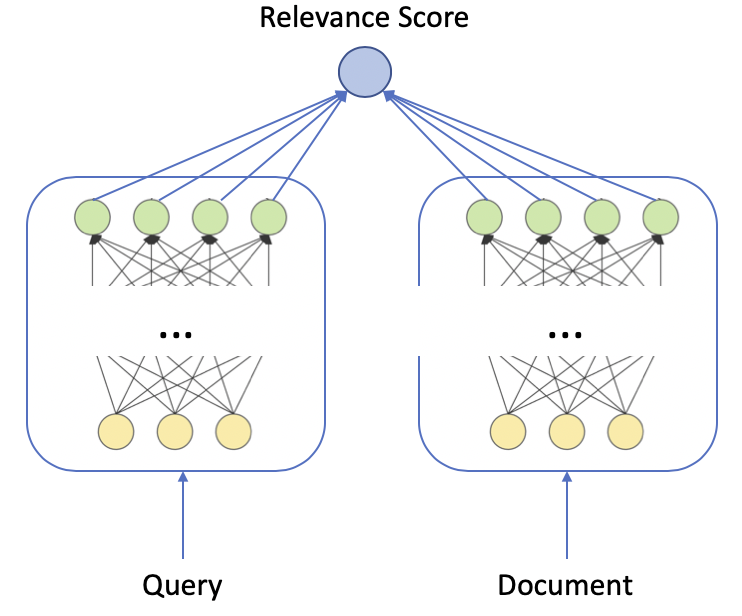
\includegraphics[width=\linewidth]{Figures/representation-based.png}
% %   \captionof{figure}{A figure}
% %   \label{fig:representation_based}
% \end{minipage}
% \begin{minipage}{.45\textwidth}
%   \centering
%   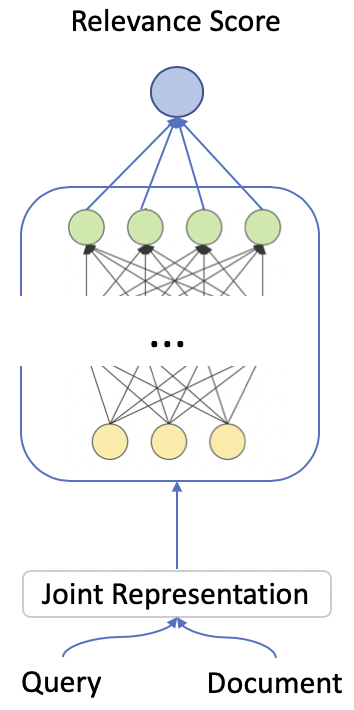
\includegraphics[width=0.5\linewidth]{Figures/interaction-based.png}
% %   \captionof{figure}{Another figure}
% %   \label{fig:interaction-based}
% \end{minipage}
% \caption{Example of \textit{representation-based} model (left) and \textit{interaction-based} model (right).}
% \label{}
% \end{figure}

\begin{figure}
    \centering
    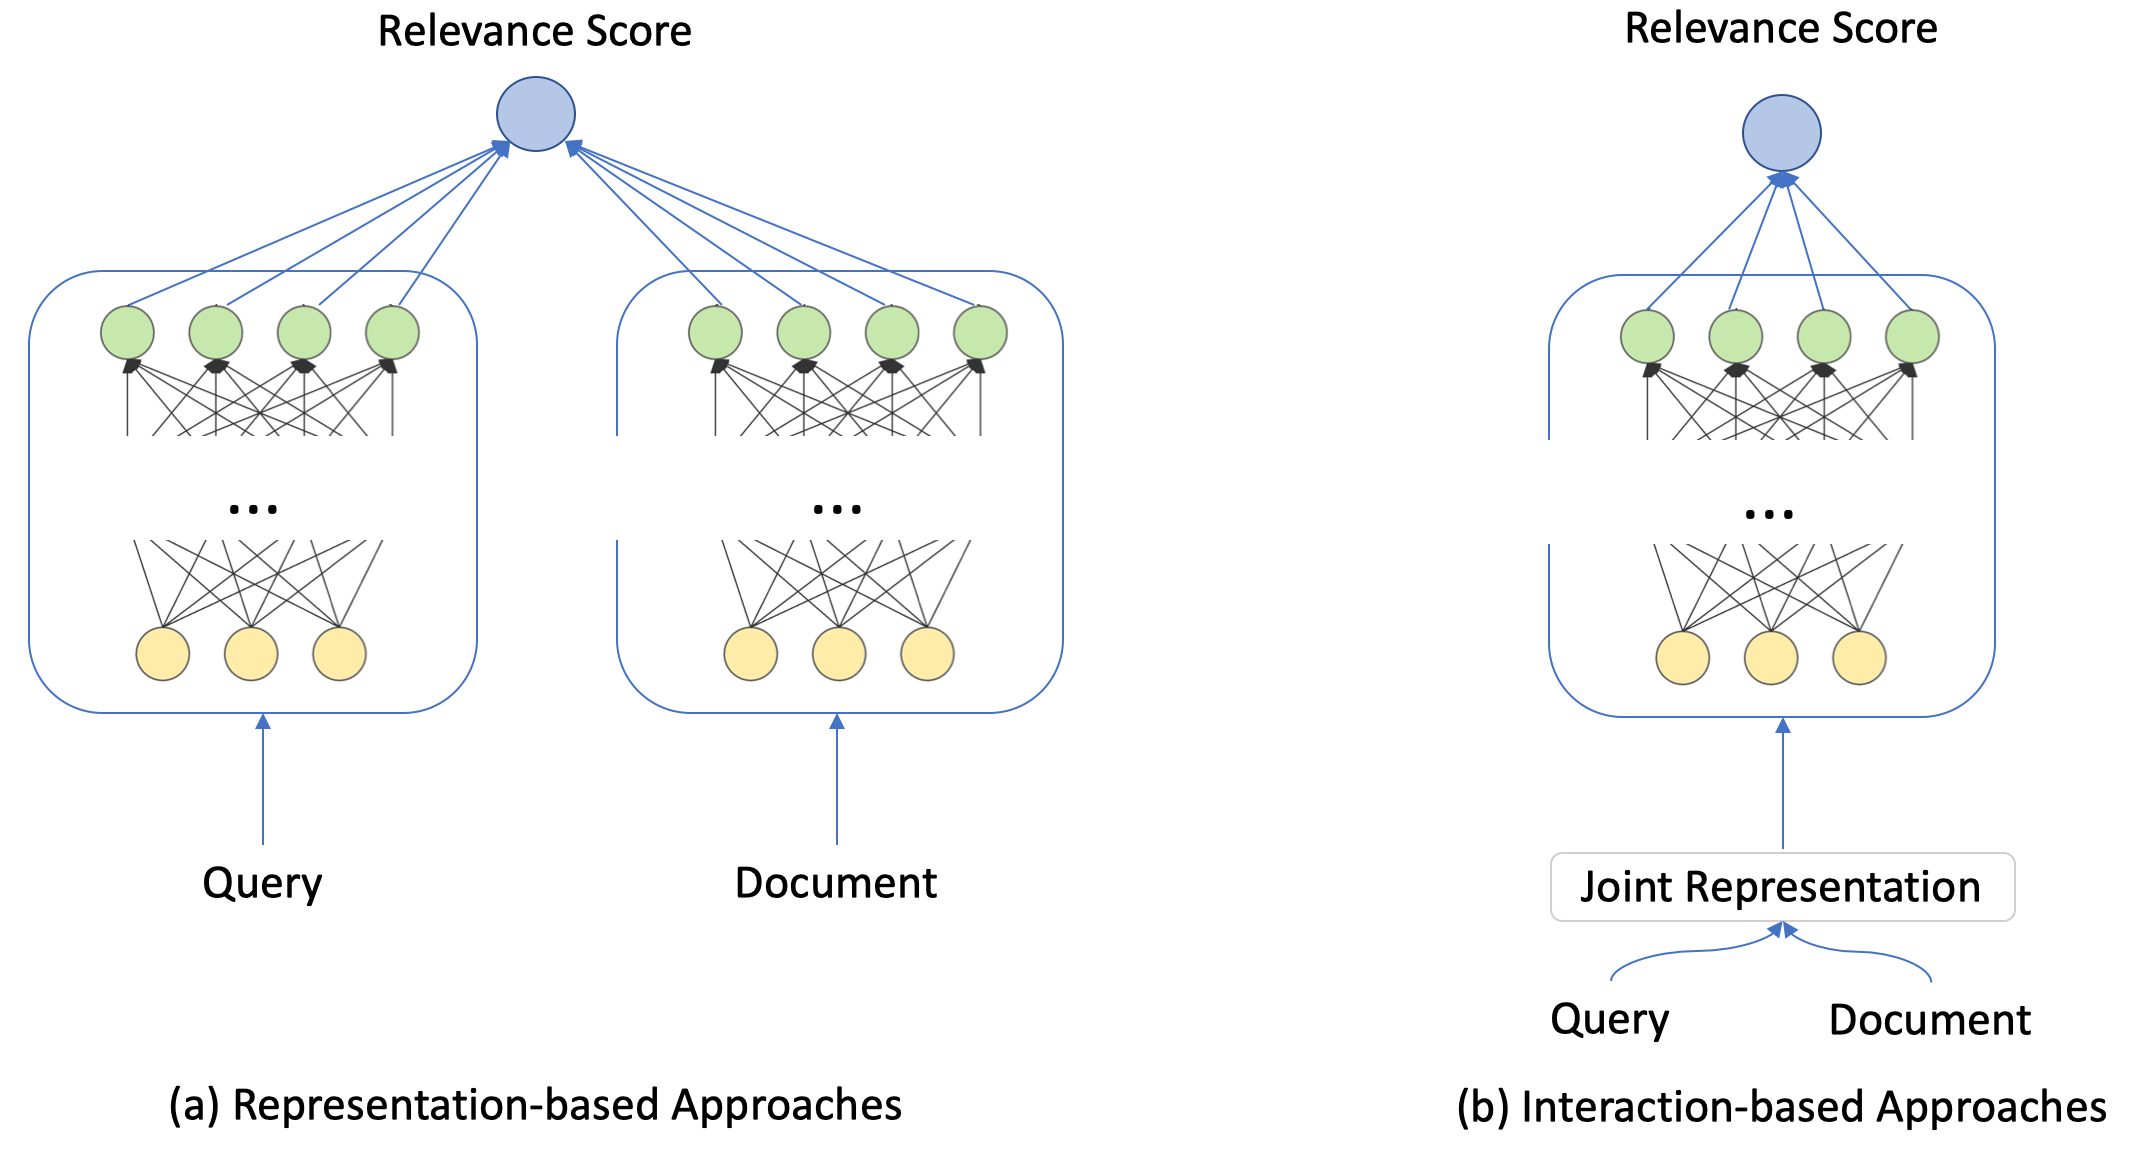
\includegraphics[width=0.7\textwidth]{Figures/neural_ir_types.png}
    \caption{Types of Neural Network Architectures for IR.}
    \label{fig:neural_ir_types}
\end{figure}

In \textit{representation-based} models (section~\ref{sec:representation_based}), the focus is on learning meaningful semantic representations of the text through several hidden layers using a deep neural network (DNN) and estimating the relevance score by using a matching function on the last level representations of the query and document. In this approach, $\Phi$ is a complex representation mapping function and $F$ is a simple matching function like cosine or dot similarity. For example, in DSSM~\citep{dssm13}, $\Phi$ is a feed forward neural network and $F$ is cosine similarity.

In \textit{interaction-based} models (section~\ref{sec:interaction_based}), the focus is on learning salient interaction patterns from the local interactions between the query and document that is fed as input into a DNN. In this approach, $\Phi$ is a simple mapping function while $F$ is a complex deep model. For example, in DRMM~\citep{Guo2016}, $\Phi$ is maps each text into a sequence of word vectors and $F$ is a feed forward neural network over the interaction matrix built from the word vectors of the two texts.

Whereas, in DUET~\citep{Mitra2017a} they combine both \textit{representation-based} and \textit{interaction-based} models by employing two separate deep neural network models--\textit{local} model that estimates the relevance score according to exact matches between query and document terms, and \textit{distributed} model that estimates relevance by matching dense lower-dimensional representations of both query and document text. The final relevance score is the sum of scores obtained from the two sub-networks. They carry out experiments on commercial search log data from Bing and compare their approach against traditional baselines (BM25, QL, DM) and neural baselines (DRMM, DSSM, CDSSM, DESM) and show that it largely outperforms the baselines. 

\subsection{Representation-Based Models}
\label{sec:representation_based}
The \textsf{Deep Structured Semantic Model} (DSSM)~\citep{dssm13} is the earliest work in neural \textit{representation-based} models for ad-hoc retrieval. The DSSM model is composed of a deep neural network with three non-linear layers on top of a word hashing layer. The query and document are first mapped to high-dimensional term vectors (\textit{bag-of-words} representation). After this the term vectors are mapped to trigram vectors by the word hashing layer, in order to cope with the large size of the vocabulary (reduces vocabulary size from 500K to 30K).

In \textsf{Convolutional Deep Structured Semantic Model} (C-DSSM)~\citep{Shen2014b} they extend DSSM by including a convolutional neural network (CNN) with max-pooling followed by a semantic layer to get high level representations of text. It first uses word hashing to project each word into a tri-gram vector. Then the convolutional layer projects each word vector within a context into a local contextual vector. Following which max-pooling is applied that picks the most salient local features to form a fixed-length global vector for queries and documents. Since both DSSM and C-DSSM fail to capture contextual information accurately,~\cite{Shen2014a} propose a \textsf{Convolutional Latent Semantic Model} (CLSM) that is built on top of DSSM. In this, the first layer consists of \textit{word-n-grams} constructed using a contextual sliding window over the input word sequence followed by letter tri-gram representation that maps each word-n-gram to its tri-gram representation like in DSSM. Then, a convolutional layer transforms these tri-grams into contextual feature vectors using a convolutional matrix shared between the word-n-grams. Then, max-pooling is applied against each dimension of the contextual feature to pick salient word-n-grams to form a fixed length vector. Finally, a semantic layer performs a non-linear transformation to obtain a semantic representation of the text. 

All of the above models are trained and evaluated on large-scale datasets from Bing. The models are discriminatively trained on query-document title pairs from the clickthrough data such that the conditional likelihood of the clicked document for a given query is maximized (\textit{cross-entropy} loss). These models are shown to outperform baselines comprising of Word Translation Model, TF-IDF, BM25 in terms of retrieval effectiveness (NDCG @1,3,10). However, in a later work~\citep{Guo2016} they show that both DSSM and C-DSSM do not perform as well as traditional IR models when using the entire document body.

In recent work~\citep{Nie_ictir18}, they compare a representation-based approach (C-DSSM without word transformation to tri-letter representation) and interaction-based approach (MatchPyramid but with additional CNN layer) under the same test conditions (experimental setup) using weak supervision~\citep{Dehghani_sigir17} (section \ref{sec:weak_supervision_ir}) with AOL query logs to generate a large amount of training data to be able to reasonably train both models on the ClueWeb09-Cat-B collection. However, their experimental results are inconsistent with that of~\cite{Dehghani_sigir17}, where they show that a neural model based on representation learning, weakly supervised by BM25, can give better retrieval effectiveness than the BM25 baseline. This could be due to the difference in dense input representation, where in~\cite{Dehghani_sigir17} they concatenate the IDF weighted element-wise sum of the term's embedding vectors of both the query and document. Finally, in~\cite{Nie_ictir18} to improve the retrieval effectiveness of the representation-based model, they employ matching at different levels of abstraction instead of a matching applied on the representation obtained from the final layer for computing a relevance score like in previous works. They build interaction matrices from the embeddings or convolved vectors between the query and document at each layer and then pick the strongest $p$ signals across each row, average it and then sum up the averages of every query representation to get a matching score for that layer. These matching scores are aggregated through a softmax gate to get a global matching score for the query and document.

In~\cite{Ai2016a,Ai2016b} they investigate the use of \textsf{PV-DBOW}~\citep{Le2014} as a document language model for retrieval. They propose three improvements over the original model for retrieval: (1) use document-frequency based rather than corpus-frequency based negative sampling so that frequent words will not be suppressed too much; (2) regularization over document representation to prevent model overfitting to short documents; and (3) joint-learning objective that considers both document-word and word-context associations to better model word substitution relations. They show higher effectiveness over LDA-based LM and QL for Robust04 and GOV2 collections.

\subsection{Interaction-Based Models}
\label{sec:interaction_based}

\subsubsection{Bag-of-words based} 
\textsf{Deep Relevance Matching Model} (DRMM)~\citep{Guo2016} is one of the first \textit{interaction-based} models to show improvements over traditional IR models (bag-of-words baselines). The query-document local interactions are first mapped into fixed-length \textit{matching histograms} to distinguish between exact matching and soft matching signals using term embedding cosine similarities. These signals are fed into a \textit{feed forward} NN and a \textit{term-gating} network that models term importance to finally get a relevance score for the query-document pair. In their experiments over Robust04 and ClueWeb-Cat-09B collections, they show significant improvements over the baselines: BM25, QL, representation-based models (DSSM, C-DSSM) and interaction-based models (MatchPyramid). The term embeddings are trained on the respective collections and they also show empirically that as the CBOW dimensions increases, the DRMM performance first increases and then slightly drops.

Similar to DRMM, \textsf{Kernel-based Neural Ranking Model} (K-NRM)~\citep{KNRM17} first creates a query-document interaction matrix that computes the cosine similarity between the term embeddings of both query and document. Then, they use multiple \textit{gaussian kernels} to obtain different levels of exact and soft-matching features from the interaction matrix which is then used as an input to a ranking layer which is a linear layer with \textit{tanh} activations to produce the final relevance score. The model is trained end-to-end using a max-margin learning-to-rank loss function. During \textit{learning}, the kernels convert the loss and adjust the word embeddings to produce a soft matching signal that better seperates relevant and irrelevant documents. They conduct extensive experiments on a Chinese commercial search engine query logs (Sogou) and show significant improvement over traditional baselines (BM25), learning-to-rank approaches (RankSVM) and neural IR baselines (DRMM, C-DSSM). They also carry out an analysis that shows using a model without multi-level soft matches or embedding learning (using pre-trained \texttt{word2vec} embeddings) quickly diminishes the performance of K-NRM.

\subsubsection{Word n-gram based}
\textsf{MatchPyramid}~\citep{matchpyramid16} is one of the first works that tries to capture hierarchical matching patterns based on \textit{n-gram} matches from the local interaction matrix of the query-document. They employ a convolutional neural network (CNN) comprising of one convolutional layer and dynamic max pooling layer on top of the interaction matrix to extract hierarchical matching patterns. Finally, the output of the CNN is fed into a MLP to produce a ranking score. They conducted extensive experiments to study the impact of pooling sizes, similarity functions (cosine, indicator, gaussian) and kernel sizes on the retrieval performance on the Robust04 collection. They achieve a better retrieval performance over traditional IR models (BM25, QL), and representation-based models (pretrained DSSM, C-DSSM), using a pooling length equivalent to paragraphs, a similarity function that differentiates between exact and semantic matches and small kernel size. 

In \textsf{Multi-level Abstraction Convolutional Model} (MACM)~\citep{Nie_ictir18, Nie_sigir_2018}, they use a model similar to MatchPyramid but with an additional convolutional and max-pooling layers and integrates the matching scores at different levels of abstraction. They determine matching scores at each abstraction level by flattening the max-pooled layer and using a MLP to obtain a score. The matching scores are aggregated through a softmax gating mechanism that considers the importance of each abstraction level by computing the max interaction values across each row of the interaction matrix or convolution feature maps and then summing up these max interaction values to get a global importance value. They show that the model trained with weak supervision using AOL query logs can outperform BM25 baseline on the ClueWeb-Cat-09B collection. They also compare with model variants without multi-level matching like in MatchPyramid and show that it outperforms these variants as well.

\textsf{Convolutional Kernel-based Neural Ranking Model} (Conv-KNRM)~\citep{ConvKNRM18} improves upon the K-NRM model by employing CNN to compose adjacent word embeddings into n-gram embeddings. The n-gram embeddings from both query and document can be combined into multiple interaction matrices that allows cross-matching of n-grams of different lengths. They then use the kernel pooling and ranking layer to combine the n-gram soft matches into a final ranking score~\citep{KNRM17}. They conducted experiments using English search logs from Bing (WSDM'09 workshop) and Chinese search logs from Sogou and show the advantages of this approach over the baselines: BM25, RankSVM, DRMM, C-DSSM, MatchPyramid and K-NRM. They also carry out experiments on ClueWeb-Cat-09B collection, where they use a domain adaptation method as there isn't sufficient training data. So, they pre-trained Conv-KNRM using the Bing search logs to be able to train the word embedding and convolutional layers effectively and then they use the relevance judgements from TREC 09-12 web tracks to re-train the soft matching kernel pooling and ranking layer keeping the embedding and convolutional layers `frozen'. This approach is shown to outperform all of the baselines mentioned above.

In \textsf{Position-Aware Convolutional Recurrent Relevance model} (PACRR)~\citep{pacrr17}, they use a combination of convolutional kernels to capture interactions that includes unigrams, bi-grams and tri-grams matches; $k$-max pooling along the query dimension to preserve important signals from different query terms; and recurrent layer to combine signals from different query terms to produce a global relevance assessment. Later, they improve on PACRR and introduce Co-PACRR~\citep{co_pacrr_wsdm18} which is a context-aware variant that takes into account the local and global context of the matching signals. For this they use three components:(1) \textit{disambiguation} component for considering the matching signal with the local context in which it occurs, this is done by introducing an input that captures the similarity between the query vector and all document contexts defined by a window; (2) \textit{cascade k-max pooling} to account for the location of matching signals by applying $k$-max pooling at multiple positions in the document instead of pooling on the entire document; (3) \textit{shuffling combination} layer to regularize the model so that it doesn't learn the absolute position of terms within the query as this could influence the aggregation layer to down-weight positions that are generally zero padded. They compare their approaches with state-of-the-art neural models including DRMM, K-NRM, local model of DUET and MatchPyramid on six years of TREC WebTrack benchmarks and show significant improvements over all baselines. They also note that their approach after re-ranking QL ranked results produce runs that are ranked within the top-3 runs on atleast 5 years based on ERR@20. %They perform an abalation analysis on the proposed components in Co-PACRR to gain insights about its usefulness. 

In~\cite{pacrr_drmm_18}, they propose several extensions to DRMM so as to account for the context in which the query terms appear. First, they introduce PACRR-DRMM a simple model that uses DRMM to independently score each of the (document-aware) query term encodings that are obtained from PACRR and aggregates these scores using a linear layer. They then propose two additional models that uses \textit{context-sensitive} term embeddings obtained from pre-trained embeddings by using a standard BiLSTM encoding scheme: (1) \textsf{Attention-Based ELement-wise} DRMM (ABEL-DRMM) in which a document representation for each q-term ($d_{q_i}$) is first computed by taking a sum of the context-sensitive encodings of d-terms, weighted by their attention score that is computed using a softmax over the dot product between that q-term and d-term encoding and then the (document-aware) q-term encoding is the hadamard product between $d_{q_i}$ and q-term encoding; (2) \textsf{POoled SImilariTy DRMM} (POSIT-DRMM) in which document-aware q-term encoding is computed by first concatenating attention scores that are obtained from cosine similarity between q-term and d-term encodings and then creating a representation that includes the max-pooled attention score and average of the $k$-max pooled attention scores. They compare against BM25, and neural IR baselines (DRMM, PACRR) on the TREC Robust04 collection and show significant improvements over all baselines.

\subsubsection{Document context based}
\textsf{DeepRank}~\citep{Pang_deeprank_2017} proposes a new architecture that better models the human judgement process while assigning relevance to a query-document pair. The model first employs a \textit{detection strategy} to extract query-centric contexts from the document, that is, the contexts with a query term in the center. Then the \textit{measure network} determines the local relevance between query and query-centric contexts by creating an 3D input tensor that includes query, and query-centric word representations along with the word-level interaction matrix between the word embeddings of the query \& query-centric context (cosine/indicator). They then use either a CNN or 2D gated recurrent unit (2D-GRU) to capture the local relevance from the input tensor producing a \textit{local relevance vector} containing matching patterns extracted from different kernels. Finally, the \textit{aggregation network} aggregates the local relevances at a query term level, and then combines it by weighting the query term importance using a term gating mechanism. The query-term level relevance is computed by first grouping the query-centric contexts that have the same query word together and then using a RNN to aggregate these local relevance vectors sequentially which also considers the position of the query-centric contexts in the document. They conduct experiments on both benchmark LETOR4.0 data (MQ2007, MQ2008) and large scale Chinese clickthrough data (Sogou). The experimental results show that: (1) Existing neural IR models such as DSSM, CDSSM, DRMM perform worse than the pairwise (RankSVM, RankBoost) and listwise (ListNet, AdaRank, LambdaMart) learning-to-rank methods using hand-crafted features; (2) DeepRank significantly improves the performance across both existing NRMs and learning-to-rank baselines.

Building upon DeepRank,~\cite{Fan_hint_2018} propose a \textsf{HIerarchical Neural maTching model} (HiNT) to learn diverse relevance patterns by a data-driven approach to allow relevance signals from different granularities (document-wide or passage-level) compete with each other to obtain a final relevance score. The model consists of two stacked components: (1) \textit{local matching layer} which produces a set of local relevance scores between a query and each passage of a document (obtained by a fixed-sized sliding window). The relevance scores are computed by building two 3D input tensors as described in ~\cite{Pang_deeprank_2017}--one for exact matching and one for semantic matching and both are given as input to a 2D Gated-RNN (spatial GRU) and the last hidden representation is taken as the matching output; (2) \textit{global matching layer} is a hybrid network that aggregates passage level relevance at different granularities--\textit{independent decision} model assumes that the passage-level relevance scores are independent and \textit{accumulative decision} model applies LSTM sequentially across the passage-level signals to generate an accumulated relevance scores at different positions. Then, $k$-max pooling is applied over the dimensions to pick the top-$k$ signals from either the passage-level or accumulated relevance signals, which is then concatenated as input to a MLP for the final relevance score. They follow a similar experimental setup as~\cite{Pang_deeprank_2017} and show improvements over traditional document-wide, passage-level retrieval models, learning-to-rank methods and neural IR models. 

In \textsf{DeepTileBars}~\citep{deeptilebars_2019}, they first split the documents into topical segments using the TextTiling algorithm~\citep{Hearst_text_tiling_94} which splits documents at positions where a change in topic is detected and they then create a query-segment interaction matrix which is fed into the neural IR  model (DeepTileBars) to obtain a relevance score. Each cell in the query-segment interaction matrix comprises of 3 values--term frequency of query word in segment, inverse document frequency of query word, and similarity score (gaussian kernel) of most similar word in the segment using word embeddings. DeepTileBars first has multiple CNNs with different kernel sizes that are employed to learn relevance patterns at different levels of granularity in the document's topic hierarchy. Then LSTMs of the same number as CNNs are used accumulate the relevance signals from the output of the CNNs, this gives relevance scores of the document at different granularities. All the different relevance scores are aggregated using a MLP to get a final global relevance score for the document. They conduct experiments on the TREC WebTrack (2010-12) and LETOR4.0 (MQ2008) and show improvements over traditional IR baselines (BM25, QL) and neural IR baselines (DRMM, MatchPyramid, DeepRank, HiNT).

\subsection{Weak Supervision for Neural IR}
\label{sec:weak_supervision_ir}
Recently, \cite{Dehghani_sigir17} propose a \textsf{weak supervision} method to use large amounts of unsupervised data to generate `weak' labels that can be used as a signal to learn neural IR models. They examined neural ranking models with different architectures, training objectives (pointwise, pairwise), and different input representations from encoding query-document pairs into sparse or dense vectors to learn dense embeddings for each text. The models are trained on billions of training examples obtained by using AOL query logs as a query set and retrieving \textit{pseudo-relevant} documents for each query using BM25 (weak supervision signal). They observed that by using just the training data obtained from the BM25 weak annotator they are able to outperform BM25 on the test dataset. This is the case only with the models that uses an embedded vector representation which concatenates the weighted element-wise sum of the term embeddings from the query and document. They also carry out analysis to understand what the model learns, if the use of pretrained embeddings from external/target corpus instead of learnt embeddings affects the performances of the models. They demonstrate that training a model with limited amount of supervised data (relevance judgements) after pre-training it on weakly supervised data gives a significant improvement in performance. This approach has been used lately to train various neural ranking models~\citep{Nie_ictir18, Nie_sigir_2018, Bo_coling18, Zamani_neural_reranking_2018}. Most recently,~\cite{Zamani_weak_sup_theory_2018} provided a theoretical foundation for explaining the successful empirical results achieved by weakly supervised neural IR models. 

``\textsf{Fidelity-Weighted Learning}''~\citep{dehghani_nips17, dehghani2018fidelityweighted} is a semi-supervised student-teacher approach for training deep neural networks with weakly supervised data instead of treating the weakly labeled samples uniformly. The \textit{student} network is initially trained on weak data to learn an initial task-dependent data representation (embedding dense vector representation in \cite{Dehghani_sigir17}). This data representation is then used with the \textit{teacher} network which is a Bayesian semi-supervised approach that learns to predict the strong data (limited relevance judgements). Then, the \textit{teacher} is used to generate a new weakly supervised data with confidence scores for each pair of data. This new weak dataset is used to fine tune the parameters of the student network. The experiments on Robust04 and ClueWeb-Cat-09B show that this approach provides improvements over the weakly supervised setup in~\cite{Dehghani_sigir17}. %The experiments on Robust04 and ClueWeb-Cat-09B, show that this approach provides significant improvements over BM25 and the weakly supervised setup in~\cite{Dehghani_sigir17}.

\subsection{Neuro-Pseudo Relevance Framework for Neural IR}
\label{sec:npr_ir}
Recently, in ~\cite{li2018nprf} they propose a \textsf{Neuro Pseudo Relevance Framework} (NPRF) that enables the use of pseudo relevance feedback with existing neural IR models. The existing neural IR models are used as scorers to evaluate the target document with respect to the top-ranked queries and the query without changing their architectures. They show two examples of the NPRF framework with two neural IR models--DRMM and KNRM, and evaluate their performance on TREC benchmark datasets (TREC 1-3, Robust04) for ad-hoc retrieval. A brief description of the architecture is given in section~\ref{sec:nprf_drmm_reproducibility_desc} and we detail the reproducibility experiments on TREC Robust04 collection that we carried out on the NPRF-DRMM variant from this paper in section~\ref{sec:nprf_drmm_reproducibility_exp}.

\subsection{Learning Sparse Representations for Indexing}

In~\citep{Zamani_neural_reranking_2018} they propose a \textsf{Standalone Neural Ranking Model} (SNRM) that can retrieve relevant documents from a large-scale collection, instead of re-ranking a small set of candidate documents that are retrieved by a first stage ranker (BM25, QL) which is the approach used in all previous neural ranking models. They propose a network architecture to learn \textit{latent sparse} representations for each continuous $n$ words of both queries and documents in the same semantic space. The learned sparse representations of n-grams are then aggregated using average pooling to get a sparse representation for the entire text. The fully connected feed forward network has a hourglass structure with small number of units in the middle layers to learn a low-dimensional representation of the data and the upper layers have a large number of units to get a sparse output representation from the sequence of $n$ embedding vectors concatenated (n-gram). These sparse representations are trained with weak supervision using a training objective that is a combination of pairwise max-margin loss and sparsity objective that minimizes the $L_1$-norm of the sparse representations. After training, the inverted index is constructed by considering each index of the learned representation ($\phi$) as a ``latent'' term, so then for each document in the collection if the $i^{th}$ index of $\phi_D$(d) is non-zero, it is added to the inverted index for the latent term $i$. During inference, the query sparse representation $\vec{q}$ is first obtained and for each non-zero element in $\vec{q}$ the corresponding documents from the inverted index are retrieved and scored using the dot product. 
% \section{Dual Embedding Space Model (DESM)}
% When using word embeddings for IR it is more appropriate to represent query terms using IN embeddings and documents terms using OUT embeddings of the trained model as it captures $aboutness$ aspect of document ranking. In this model\citep{Nalisnick:2016,Mitra2016a}, word2vec is trained on search queries instead of document body text as it empirically performs better. Training on short queries makes inter term similarity more pronounced when using both terms represented as IN vectors. While using IN-OUT vectors for terms gives a better topical notion of relatedness which is better for retrieval.

% The \textit{Continuous Bag-of-Words} (CBOW) model~\citep{Mikolov2013} with negative sampling is used to learn the word embeddings as its able to capture word co-occurrences. The model predicts word $w_i$ by adapting its representation vector such that it has a large inner product with the mean of the context word vectors.

% The ranking function based on the learnt embeddings is defined as
% \begin{align}
%     DESM(Q,D) = \
%     \frac{1}{|Q|}\sum_{q_i \in Q}{}\frac{ q_i^T{\bar{D}}}{\|q_i\|\|{\bar{D}}\|} \\
%     \intertext{where}
%     \bar{D} = 
%     \frac{1}{|D|}\sum_{d_j \in D}{}\frac{d_j}{\|d_j\|}
% \end{align}

% Here $\bar{D}$ is the centroid of all the normalized vectors for the words in the document which represents a single embedding for the whole document.

% \textbf{Training corpus}. The CBOW model is trained on a query corpus consisting of 6 million queries and having a vocabulary size of 2.7 million words. All experiments are repeated using another CBOW model trained on document body text with 341 million distinct sentences sampled from Bing search index having a vocabulary of 5.1 million words.

%-----------------------------------------------------
%	SECTION 3
%-----------------------------------------------------
% \section{DUET Architecture}
% A document ranking model composed of two separate deep neural networks, one that matches query and document using local representations (local model) and one that matches them using distributed representations (distributed model)~\citep{Mitra2017a}. Both these deep neural networks are jointly trained as part of a single neural network. The final score under the architecture is the sum of scores from individual networks,
% \begin{equation}
%     f(Q,D) = f_l(Q,D) + f_d(Q,D)
% \end{equation}
% where query and document are ordered list of terms, Q = [$q_1,...,q_{n_q}$] and D = [$d_1,...d_{n_d}$]. Each term is represented as a one-hot vector of $m_l$ dimension, where $m_l$ is the size of the vocabulary. The length of the inputs across all queries and documents are fixed, such that, only the first 10 terms in the query and first 1000 terms in the document are considered.
% \begin{figure*}
%     \centering
%     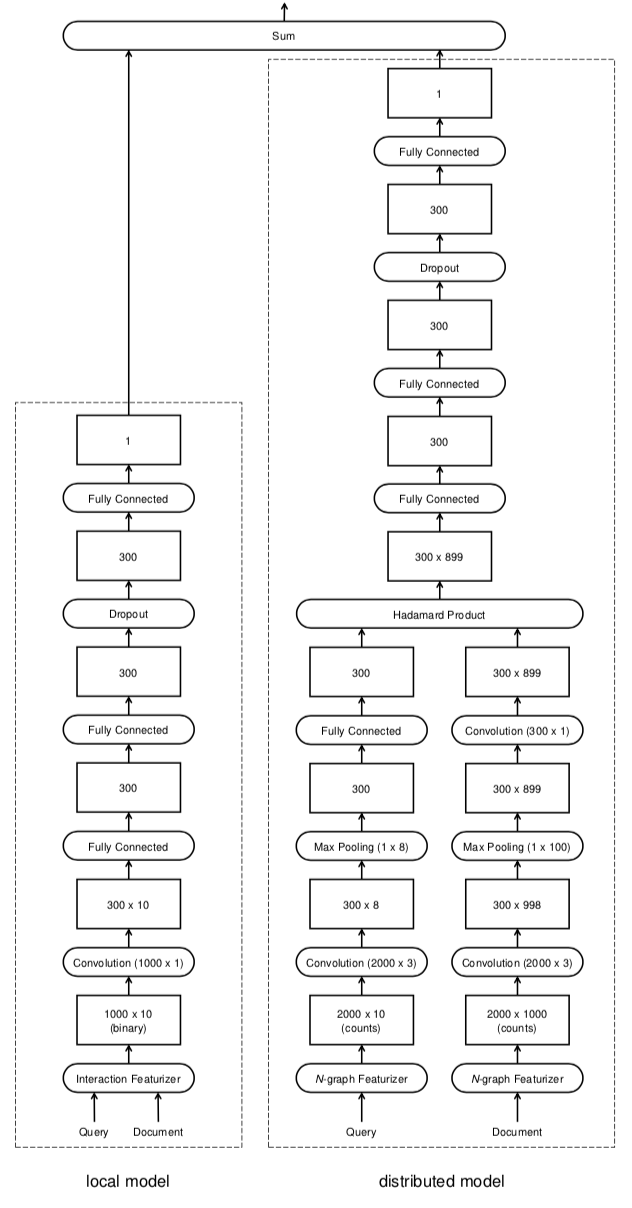
\includegraphics{Figures/DUET.png}
%     \caption{DUET architecture. The local model takes query-document interaction matrix as input, whereas distributed model learns embeddings of query and document text before matching. The parameters of both models are jointly optimised.}
%     \label{fig:duet_architecture}
% \end{figure*}

% \textbf{Local Model}. The model estimates document relevance based on exact matching patterns between query terms in the document. The interaction matrix is a $n_d * n_q$ binary matrix $X = D^TQ$, that captures every exact match of query terms in the document. The matrix is passed through a convolutional layer with $c$ filters, a kernel size $n_d * 1$ and stride of 1. The output $Z$ of the convolutional layer (eq.~\ref{eq:conv_layer_eq_duet}) is then passed through two fully connected layers, a dropout layer and a final fully-connected layer that gives a single score. All nodes in the local model uses hyperbolic tangent for non-linearity.
% \begin{align}\label{eq:conv_layer_eq_duet}
%     \mathrm{Z_i} = \tanh(\mathrm{X}_i^T\mathrm{W})
% \end{align}
% where W is $n_d * c$ matrix of learnable parameters.

% \textbf{Distributed Model}. This model learns a dense lower-dimension vector representations of both query and document, before computing the positional similarity between them in the embedding space. Character $n$-graph based representation of each term in the query and document is used. For each term, all the $n$-graphs present for $1 \leq n \leq G$ is counted, where G is set to 5. This $n$-graph frequency vector of length $m_d$ is used to represent the term ($m_d = 2000$, which is the top-2000 most popular $n$-graphs).

% In this model, the $Q$ matrix $m_d*n_q$ and $D$ matrix $m_d*n_d$ are sent to a convolutional layer of window ($m_d*3$) and filter size of 300. This layer generates a tensor of dimension $300*8$ for the query, and $300*998$ for the document. Following this there is max-pooling layer. For the query, the pooling kernel dimension is $1*8$, to get one query matrix $\widetilde Q$ ($300*1$). For the document, the pooling kernel is $1*100$ to generate a matrix $\widetilde D$ ($300*899$). The window based max pooling strategy helps distinguish between matches in different parts of the document. The combination of convolutional, max-pooling and fully-connected layers enables the model to learn suitable representations of text for effective inexact matching. Finally the matching is performed using an element-wise product between embedded document matrix and broadcasted query embedding.
% \begin{align*}
%     \widetilde X = (\underbrace{\widetilde Q...\widetilde Q}_\text{899 times})\circ\widetilde D
% \end{align*}

% \textbf{Training Objective}. Each training sample consists of a query, relevant document and set of non-relevant documents. Softmax function is used to compute posterior probability of relevant document given a query based on the score.
% \begin{align*}
%     p(D^*|Q) = \frac{\exp (f(Q,D^*))}{\sum_{D \in N} \exp (f(Q,D))}
% \end{align*}

% \begin{sidewaystable}
%     % \centering
%     \footnotesize
%     \scalebox{0.65}{
%     \begin{tabular}{m{5em}m{7em}m{7em}m{7em}m{7em}m{7em}m{7em}m{7em}m{7em}m{7em}m{7em}m{7em}m{7em}}
%     \toprule
%          & DESM & DUET & DSSM & CDSSM & DRMM & MatchPyramid & PACRR \newline Co-PACRR & K-NRM & MACM & Conv KNRM & DeepRank & FNRM \newline \cite{Dehghani_sigir17}\\
%          \midrule
%         I/P Repr. & BOW\newline+\newline Embeddings & query-doc interaction matrix \newline query and doc tri-gram vector & Bag-of-character tri-gram vector & Bag-of-character tri-gram vector & query-doc interaction matrix (cosine) &
%         query-doc interaction matrix (cosine, ind.,\newline dot, gaussian) &
%         query-doc interaction matrix (cosine) & query-doc interaction matrix (cosine) & query-doc interaction matrix (cosine)\\
%         \addlinespace[1em]
        
%         Training workload & --- & click-through data \newline 200K Bing & click-through data \newline 16K Bing & click-through data \newline 16K Bing & judgements \newline Robust04 Track \newline CW WebTrack 09-11 & judgements \newline Robust04 Track & judgements \newline CW \newline WebTrack 09-14 & click-through data 100K Sogou (Chinese) & AOL query logs (weak sup.)\\
%         \addlinespace[1em]
        
%         Word Embeddings & \texttt{CBOW} \& \texttt{SGNS} Bing & --- & --- & --- & \texttt{CBOW} \newline Robust04 & \texttt{Glove} Wikipedia & \texttt{word2vec} GoogleNews & --- & \texttt{Glove} Wikipedia\\
%         \addlinespace[1em]
        
%         Evaluation Testset & Bing Prop. \newline Robust04, CW & Bing Prop. & Bing Prop. & Bing Prop. & Robust04, CW & Robust04 titles & CW WebTrack 09-14 & Sogou Prop. & CW WebTrack 09-12\\
%         \addlinespace[1em]
        
%         Impl. Trainable & \checkmark & weak sup. & weak sup. & weak sup. & \checkmark & \checkmark & \checkmark & \checkmark & weak sup.\\
%         \addlinespace[1em]
        
%         OOV \newline handling & skips & \xmark & \xmark & \xmark & Ind. match 1/0 & NA. & Retrain unseen words & \xmark & skips\\
%         \addlinespace[1em]
        
%         Baselines & BM25, LSA & BM25, LSA, \newline QL, DRMM, \newline DSSM, CDSSM, DESM & BM25, LSA, \newline DAE & BM25, LSA,\newline DSSM & QL, BM25, \newline DSSM, CDSSM, MP & QL, BM25, \newline DSSM, CDSSM & DUET-L, KNRM, DRMM, MP & BM25, QL, \newline DSSM, CDSSM, \newline DRMM, RankSVM & BM25, QL\\
%         %\addlinespace[1cm]
        
%         Training Obj. & --- & log-likelihood & cross entropy & cross entropy & max margin & max margin & max margin \newline Co-PACRR (cross entropy) & max margin & max margin\\
%     \bottomrule
%     \end{tabular}}
%     \caption{Comparison of Neural IR model architectures and experimental setups.}
%     \label{tab:neuir_comparison}
% \end{sidewaystable}

% \pagebreak
{
    \centering
    \tiny
    % \scalebox{0.63}{
    %{lm{7em}m{7em}m{7em}m{7em}m{7em}m{5em}m{7em}m{5em}}
    \begin{longtable}{C{3.7em}m{7em}C{5em}C{4em}m{4.5em}C{4.2em}C{3.5em}m{7.1em}L{3.5em}}
    \addlinespace[1em]
    \toprule
    \addlinespace[2em]
    \caption[]{Comparison of Neural IR model architectures and experimental setups. (continued)}
    \endfoot
    \caption{Comparison of Neural IR model architectures and experimental setups.}
    \endlastfoot
    \toprule
    Model & I/P Repr. & Training workload & Word \newline Embeddings & Evaluation Testset & Impl. Trainable & OOV \newline handling & Baselines & Training Obj.\\
    \midrule
    \endhead
        
        DESM & BOW +\newline Embeddings & --- & \texttt{CBOW} \& \texttt{SGNS} Bing & Bing Prop., \newline Robust04, CW & \checkmark & skips & BM25, LSA & ---\\
        \addlinespace[0.5em]
        \midrule
        \addlinespace[0.5em]
        
        DUET & query-doc interaction matrix \newline query \& doc \newline tri-gram vector & click-through data \newline 200K Bing & --- & Bing Prop. & weak sup. & \xmark & BM25, LSA, \newline QL, DRMM, \newline DSSM, CDSSM, DESM & log-likelihood\\
        \addlinespace[0.5em]
        \midrule
        \addlinespace[0.5em]
        
        DSSM & Bag-of-character tri-gram vector & click-through data \newline 16K Bing & --- & Bing Prop. & weak sup. & \xmark & BM25, LSA, \newline DAE & cross \newline entropy\\
        \addlinespace[0.5em]
        \midrule
        \addlinespace[0.5em]
        
        CDSSM & Bag-of-character tri-gram vector & click-through data \newline 16K Bing & --- & Bing Prop. & weak sup. & \xmark & BM25, LSA, \newline DSSM & cross \newline entropy\\
        \addlinespace[0.5em]
        \midrule
        \addlinespace[0.5em]
        
        DRMM & query-doc interaction matrix (cosine) & judgements \newline Robust04, CW WebTrack 09-11 & \texttt{CBOW} \newline Robust04 & Robust04, CW & \checkmark & Ind. match 1/0 & QL, BM25, \newline DSSM, CDSSM, MP & max \newline margin\\
        \addlinespace[0.5em]
        \midrule
        \addlinespace[0.5em]
        
        MatchPyr. MP & query-doc interaction matrix (cosine, ind., dot, gaussian) & judgements Robust04 & \texttt{Glove} Wikipedia & Robust04 titles & \checkmark & NA.\footnote{Not mentioned in the paper.} & QL, BM25, \newline DSSM, CDSSM & max \newline margin\\
        \addlinespace[0.5em]
        \midrule
        \addlinespace[0.5em]
        
        PACRR \newline Co-PACRR & query-doc interaction matrix (cosine) & judgements CW WebTrack 09-14 & \texttt{word2vec} GoogleNews & CW WebTrack 09-14 & \checkmark & Retrain OOV words & DUET-L, KNRM, DRMM, MP & max \newline margin \newline Co-PACRR (cross entropy)\\
        \addlinespace[0.5em]
        % \midrule
        % \addlinespace[0.5em]
        
        K-NRM & query-doc interaction matrix (cosine) & click-through data 100K Sogou (Chinese) & Trained with model & Sogou Prop. & weak sup. & \xmark & BM25, QL, \newline DSSM, CDSSM, DRMM, RankSVM & max \newline margin\\ 
        \addlinespace[0.5em]
        \midrule
        \addlinespace[0.5em]
        
        Conv-KNRM & query term embed matrix \& doc term embed matrix & click-through data \newline 100K Sogou, \newline 100K Bing, \newline CW 09-12 & Trained with model & Sogou Prop., \newline Bing Prop.,\newline CW 09-12 & weak sup. & \xmark & BM25, MP,\newline DRMM, CDSSM, KNRM, RankSVM & max \newline margin\\
        \addlinespace[0.5em]
        \midrule
        \addlinespace[0.5em]
        
        MACM & query-doc interaction matrix (cosine) & AOL query logs \newline (weak sup.) & \texttt{Glove} Wikipedia & CW 09-12 & weak sup. & skips & BM25, QL & max \newline margin\\
        \addlinespace[0.5em]
        \midrule
        \addlinespace[0.5em]
        
        FNRM \newline \cite{Dehghani_sigir17} & query \& doc weighted avg. embedding repr. & AOL query logs & \texttt{word2vec} GoogleNews & Robust04, CW 09-12 & weak sup. & \xmark & BM25 & max \newline margin\\
        \addlinespace[0.5em]
        \midrule
        \addlinespace[0.5em]
        
        DeepRank & 3D tensor of query, query-centric word repr. \& interaction matrix & LETOR4.0 (MQ2007 \& MQ2008), click-through data (Sogou) & \texttt{CBOW} Wikipedia & LETOR4.0, \newline Sogou Prop. & \checkmark & NA. & BM25-Title, RankSVM, RankBoost, ListNet, AdaRank, LambdaMart, DSSM, CDSSM, DRMM, MP & max \newline margin\\
        \addlinespace[0.5em]
        \midrule
        \addlinespace[0.5em]
        
        HiNT & 3D tensor of query, passage word repr. \& interaction matrix & LETOR4.0 (MQ2007 \& MQ2008) & \texttt{CBOW} Wikipedia & LETOR4.0 & \checkmark & rand. sample (-0.02, 0.02) & BM25, AdaRank, LambdaMart, DSSM, DRMM, Duet, DeepRank & max \newline margin\\
        \addlinespace[0.5em]
        \midrule
        \addlinespace[0.5em]
        
        DeepTileBars & 3D tensor of query-segment interaction matrix (\textit{tf}, \textit{idf}, \textit{gaussian sim.}) & judgements \newline CW WebTrack 10-12 & \texttt{word2vec} GoogleNews & CW 10-12, LETOR4.0 (MQ2008) & \checkmark & NA. & BM25, QL, \newline DRMM, MP, \newline HiNT, DeepRank & cross \newline entropy\\
        \addlinespace[0.5em]
        \midrule
        \addlinespace[0.5em]
        
        SNRM \cite{Zamani_neural_reranking_2018} & query and doc sparse embeddings (BOW) & AOL query logs (weak sup.) & \texttt{Glove} Wikipedia & Robust04, CW 09-12 & weak sup. & \xmark & QL, SDM, RM3, FNRM, CDSSM & max margin + $L_1$-norm sparsity obj.\\
        \bottomrule
    
    \label{tab:neuir_comparison}
    \end{longtable}
    % }
}


%-----------------------------------------------------
%	SECTION 7
%-----------------------------------------------------
%\section{IRGAN}

% \begin{figure*}
%     \centering
%     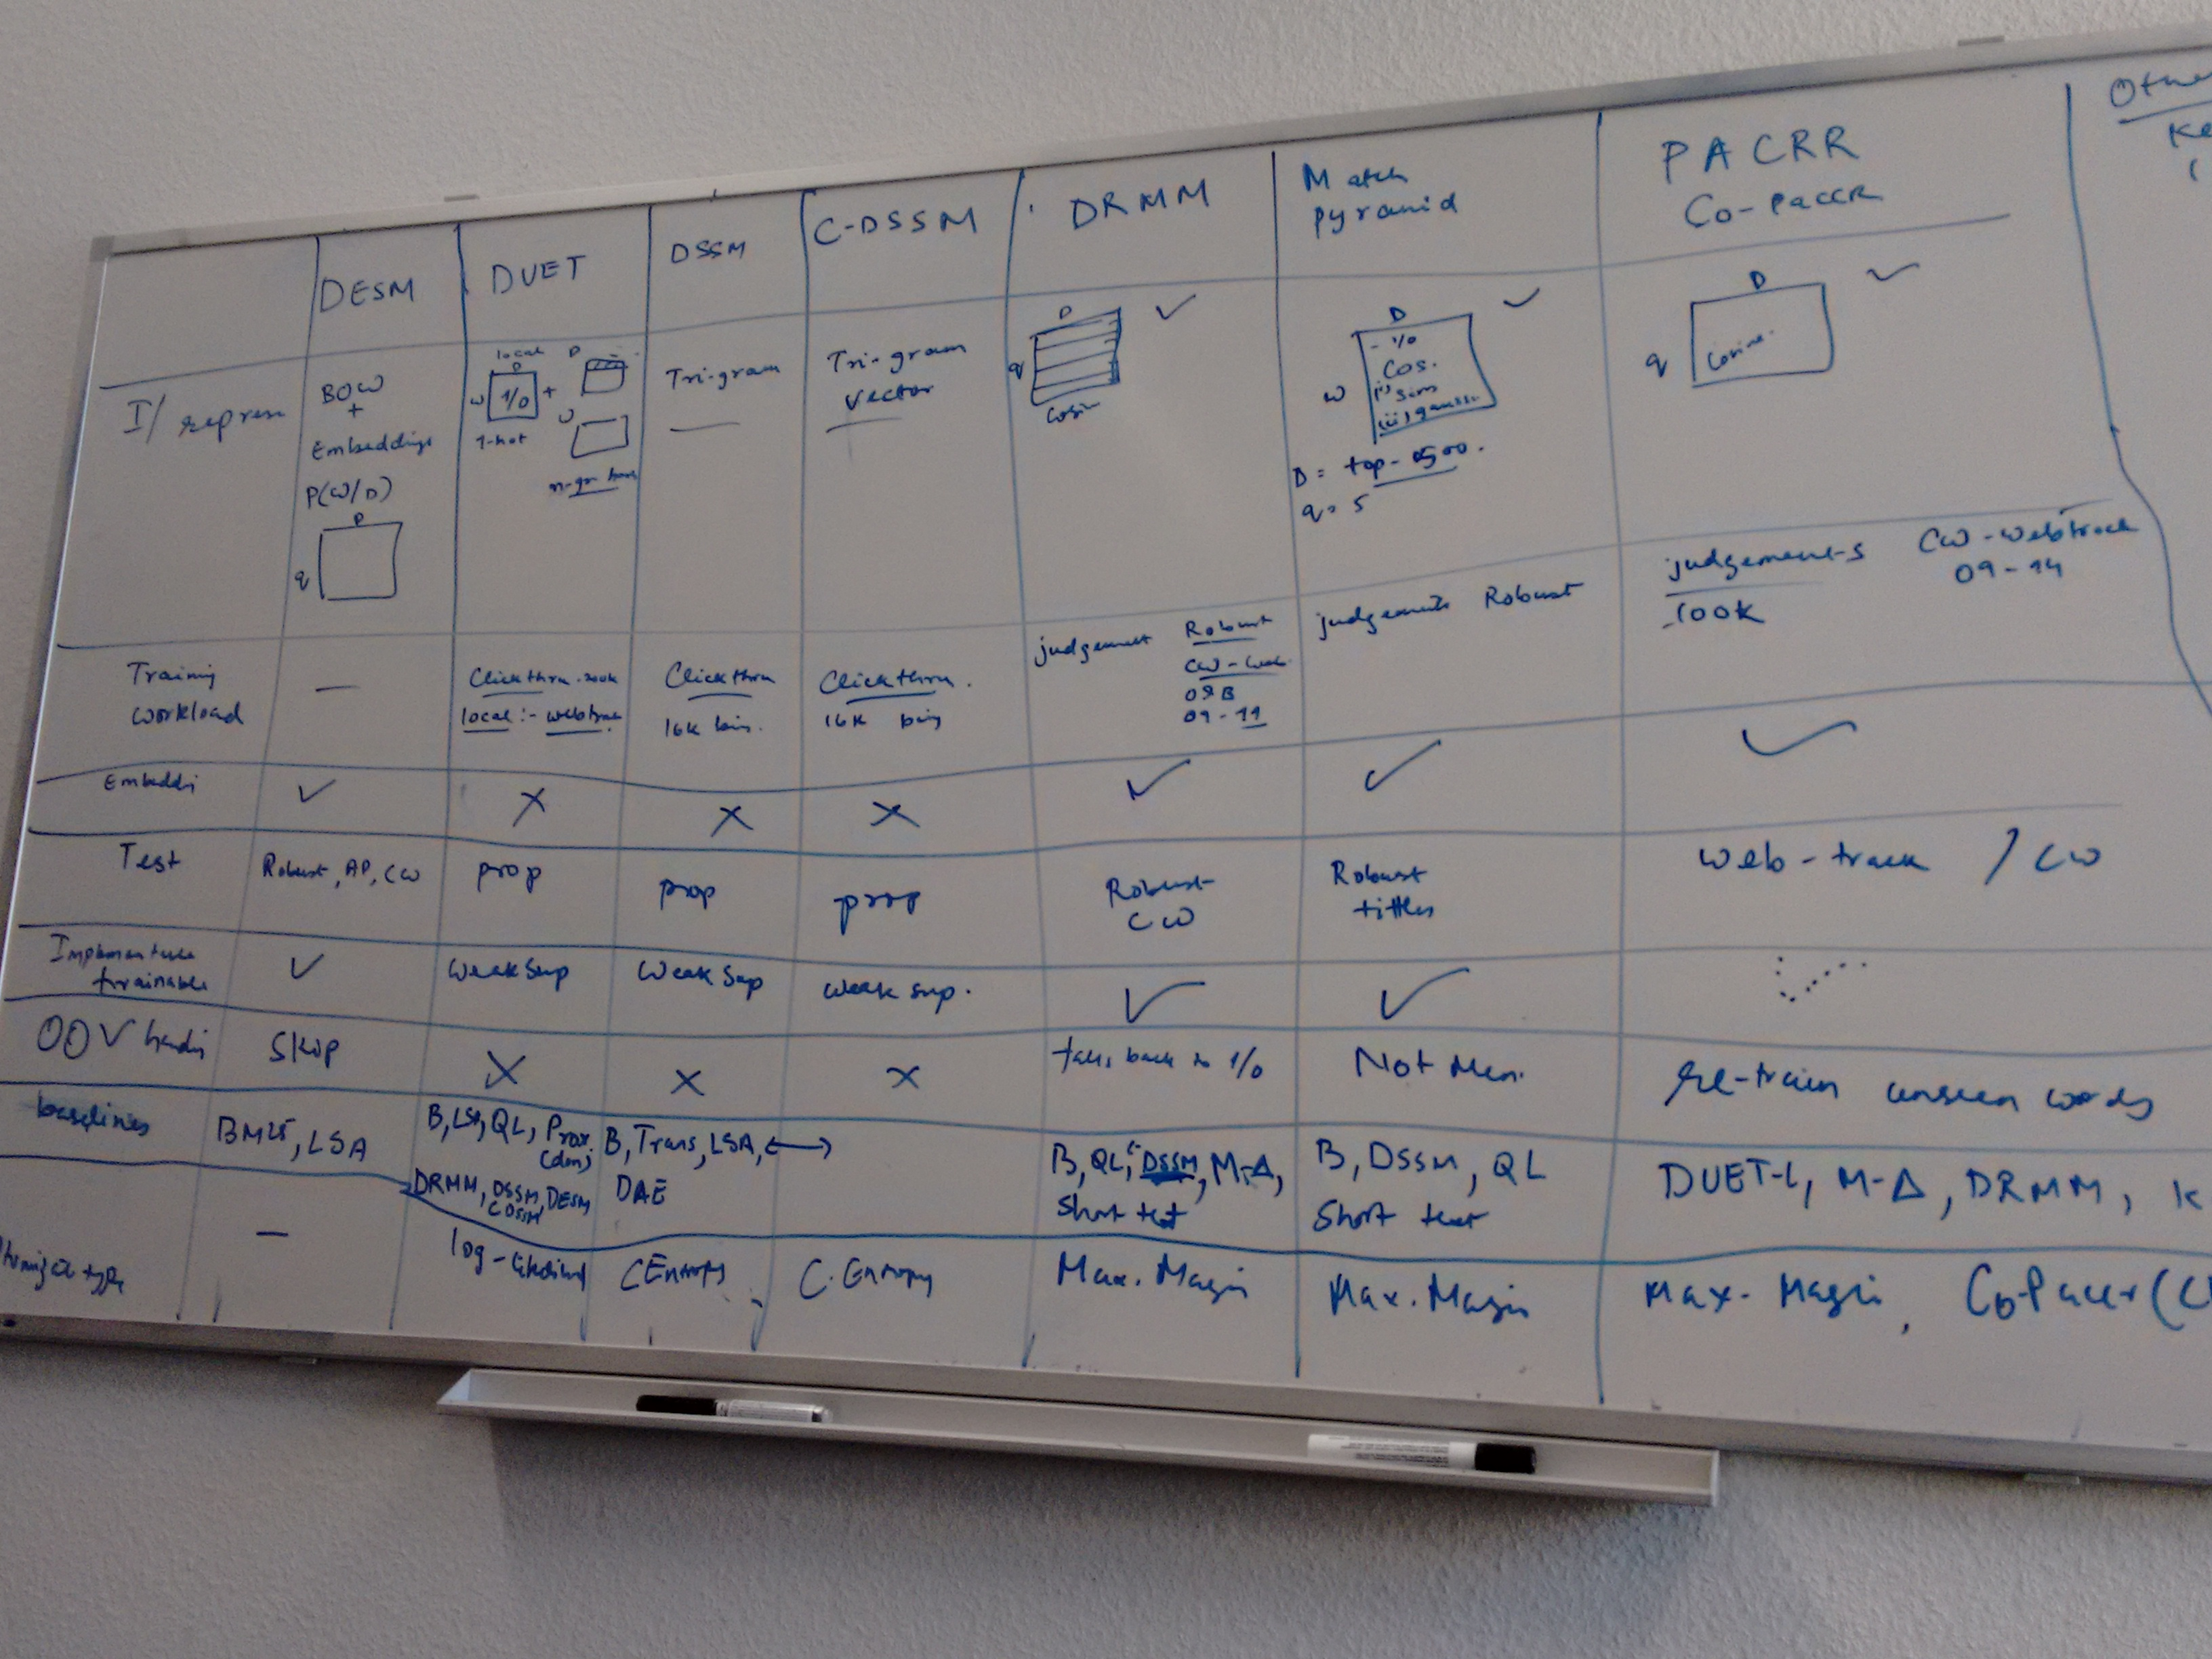
\includegraphics[width=\textwidth]{Figures/model_compare.jpg}
%     \caption{Comparison of model architectures.}
%     \label{fig:models_comparison}
% \end{figure*}

\section{Interpretability in ML}
\label{sec:interpretability_ml}

There are two main approaches to interpretability in machine learning models: {\it model agnostic} and {\it model introspective} approaches. Model agnostic approaches \citep{Ribeiro16, Ribeiro18} generate post-hoc explanations for the original model by treating it as a black box by learning an interpretable model on the output of the model or by perturbing the inputs or both. Model introspective approaches on one hand include ``interpretable'' models such as decision trees \citep{letham2015}, attention-based networks \citep{Xu2015}, and sparse linear models \citep{Ustun2016} where there is a possibility to inspect individual model components (path in a decision tree, feature weights in linear models) to generate useful explanations. On the other hand, there are gradient-based methods like \cite{Simonyan2013DeepIC} that generates attributions by considering the partial derivative of the output with respect to the input features. Following this, there were many works \citep{Lundberg17, ShrikumarGK17, Bach15, Arras17} that generate attributions by inspecting the neural network architectures.  

\subsection{Interpretability in Ranking Models}
\label{sec:interpretability_in_ir}

Recently there have been few works focused on interpretability \citep{Singh19} and diagnosis of neural IR models \citep{Rennings19, PangLG0C17, Cohen18}. In the diagnostic approaches, they use the formal retrieval constraints (``axioms'') defined for traditional retrieval models to find the differences between neural IR and learning-to-rank approaches with hand-crafted features through a manual error analysis \citep{PangLG0C17} or build diagnostic datasets based on the axioms to empirically analyse these models \citep{Rennings19}. Also, in~\cite{Cohen18} they take a diagnostic approach by probing neural retrieval models by taking each layers weights and using it as an input to a classifier for different types of NLP tasks (sentiment analysis, POS tagging, etc.). The performance on those tasks would provide insight into the type of information encoded in each layer. 

Whereas, in \cite{Singh19} they built a \textsf{Explainable Search System} (EXS) that adapts a local model agnostic interpretability approach (LIME)~\citep{Ribeiro16} to explain the relevance of a document for a query for various neural IR models (DESM, DRMM). They provide visual explanations that also helps answer why one document is ranked higher than another or what is the intent of the query according to the neural ranker. 
